\chapter{CƠ SỞ LÝ THUYẾT VÀ CÔNG NGHỆ SỬ DỤNG}
\section{Trí tuệ nhân tạo (Artificial Intelligence)}

Trí tuệ nhân tạo (Artificial Intelligence - AI) là lĩnh vực nghiên cứu thuộc khoa học máy tính nhằm xây dựng các hệ thống có khả năng mô phỏng trí thông minh của con người. AI cho phép máy tính thực hiện nhiều nhiệm vụ như học tập, suy luận, lập kế hoạch, xử lý ngôn ngữ tự nhiên, nhận dạng hình ảnh và đưa ra quyết định.

Trong những năm gần đây, AI phát triển mạnh nhờ sự gia tăng về năng lực tính toán, dữ liệu lớn (Big Data) và các mô hình học sâu (Deep Learning). AI đã được ứng dụng rộng rãi trong nhiều lĩnh vực như giáo dục, tài chính, thương mại điện tử, y tế, giao thông và dịch vụ khách hàng.

Trong đề tài này, AI đóng vai trò là nền tảng giúp hệ thống Chatbot hiểu câu hỏi của người dùng, truy xuất thông tin từ tài liệu và sinh ra câu trả lời phù hợp.

\section{Mô hình ngôn ngữ lớn (Large Language Model)}

Large Language Model (LLM) là các mô hình học sâu được huấn luyện trên tập dữ liệu văn bản rất lớn nhằm hiểu và sinh ngôn ngữ tự nhiên.

LLM có khả năng:

\begin{itemize}
	
	\item Trả lời câu hỏi.
	
	\item Tóm tắt văn bản.
	
	\item Dịch ngôn ngữ.
	
	\item Sinh mã nguồn.
	
	\item Phân tích tài liệu.
	
	\item Hội thoại với người dùng.
	
\end{itemize}

Các mô hình phổ biến hiện nay gồm GPT, Llama, Gemini, Claude, Qwen,...

Trong dự án, LLM chịu trách nhiệm tạo ra câu trả lời cuối cùng sau khi nhận được dữ liệu liên quan từ hệ thống Retrieval.

\section{Retrieval-Augmented Generation (RAG)}

Retrieval-Augmented Generation (RAG) là kỹ thuật kết hợp giữa truy xuất dữ liệu (Retrieval) và mô hình sinh ngôn ngữ (Generation).

Thay vì chỉ dựa vào kiến thức đã được huấn luyện trước, hệ thống sẽ tìm kiếm các đoạn tài liệu liên quan trước khi gửi vào mô hình AI.

Quy trình hoạt động gồm các bước:

\begin{enumerate}
	
	\item Người dùng gửi câu hỏi.
	
	\item Câu hỏi được chuyển thành Vector Embedding.
	
	\item Hệ thống tìm kiếm các đoạn văn bản tương đồng trong ChromaDB.
	
	\item Các đoạn tài liệu được đưa vào Prompt.
	
	\item LLM sinh câu trả lời dựa trên tài liệu vừa truy xuất.
	
\end{enumerate}

Nhờ đó, câu trả lời luôn bám sát tài liệu môn học và giảm hiện tượng Hallucination.

\section{Fine-Tuning}

Fine-Tuning là quá trình huấn luyện tiếp một mô hình ngôn ngữ đã được huấn luyện trước bằng tập dữ liệu chuyên biệt.

Mục tiêu của Fine-Tuning là giúp mô hình:

\begin{itemize}
	
	\item Hiểu ngữ cảnh chuyên ngành.
	
	\item Trả lời đúng theo dữ liệu huấn luyện.
	
	\item Tăng độ chính xác.
	
	\item Giảm câu trả lời sai.
	
\end{itemize}

Trong đề tài, nhóm tiến hành nghiên cứu Fine-Tuning trên dữ liệu môn học nhằm so sánh hiệu quả với phương pháp RAG.

\section{Embedding}

Embedding là kỹ thuật chuyển đổi văn bản thành vector số có nhiều chiều.

Các vector này phản ánh ý nghĩa ngữ nghĩa của văn bản thay vì chỉ dựa vào từ khóa.

Quá trình Embedding trong hệ thống bao gồm:

\begin{enumerate}
	
	\item Đọc tài liệu PDF.
	
	\item Chia nhỏ thành nhiều đoạn (Chunk).
	
	\item Sinh Vector Embedding.
	
	\item Lưu Vector vào ChromaDB.
	
	\item Khi người dùng hỏi, câu hỏi cũng được chuyển thành Vector.
	
	\item So sánh độ tương đồng Cosine Similarity.
	
\end{enumerate}

Embedding giúp tăng tốc độ truy xuất và cải thiện độ chính xác của hệ thống.

\section{ChromaDB}

ChromaDB là cơ sở dữ liệu Vector mã nguồn mở dùng để lưu trữ Embedding.

Khác với cơ sở dữ liệu truyền thống chỉ lưu dữ liệu dạng bảng, ChromaDB lưu các Vector có hàng trăm hoặc hàng nghìn chiều.

Trong hệ thống, ChromaDB thực hiện:

\begin{itemize}
	
	\item Lưu trữ Embedding.
	
	\item Tìm kiếm Vector gần nhất.
	
	\item Truy xuất các đoạn tài liệu liên quan.
	
	\item Trả về dữ liệu cho mô hình AI.
	
\end{itemize}

Việc sử dụng ChromaDB giúp hệ thống tìm kiếm dữ liệu nhanh và chính xác ngay cả khi số lượng tài liệu lớn.

\section{FastAPI}

FastAPI là Framework phát triển REST API bằng ngôn ngữ Python.

Các ưu điểm của FastAPI gồm:

\begin{itemize}
	
	\item Hiệu năng cao.
	
	\item Dễ xây dựng API.
	
	\item Tự sinh Swagger Documentation.
	
	\item Hỗ trợ Async.
	
	\item Dễ tích hợp AI.
	
\end{itemize}

Trong đề tài, FastAPI đảm nhiệm:

\begin{itemize}
	
	\item Nhận câu hỏi từ Frontend.
	
	\item Gọi ChromaDB.
	
	\item Gọi mô hình AI.
	
	\item Trả kết quả cho React.
	
	\item Quản lý Upload PDF.
	
\end{itemize}

\section{ReactJS}

ReactJS là thư viện JavaScript được Meta phát triển nhằm xây dựng giao diện người dùng theo mô hình Component.

React giúp:

\begin{itemize}
	
	\item Giao diện hiện đại.
	
	\item Cập nhật dữ liệu theo thời gian thực.
	
	\item Dễ mở rộng.
	
	\item Tái sử dụng Component.
	
\end{itemize}

Trong hệ thống, ReactJS được sử dụng để xây dựng giao diện Chatbot, quản lý tài liệu và hiển thị kết quả so sánh giữa RAG và Fine-Tuning.

\section{Kiến trúc tổng thể hệ thống}

Hinh \ref{fig:context} mô tả kiến trúc tổng thể của hệ thống Chatbot hỗ trợ học tập.

\begin{figure}[H]
	\centering
	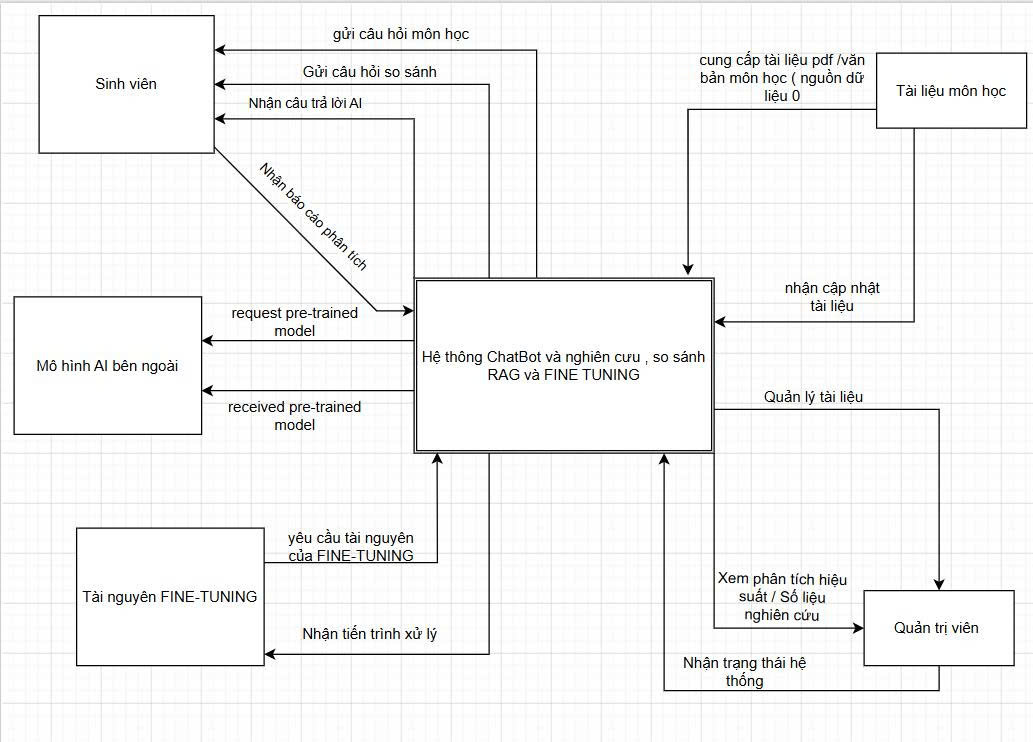
\includegraphics[width=0.95\textwidth]{images/context.png}
	\caption{Kiến trúc tổng thể hệ thống}
	\label{fig:context}
\end{figure}

Kiến trúc hệ thống gồm năm thành phần chính:

\begin{itemize}
	
	\item Người dùng (Sinh viên).
	
	\item Quản trị viên.
	
	\item Hệ thống Chatbot.
	
	\item Kho tài liệu môn học.
	
	\item Mô hình AI và tài nguyên Fine-Tuning.
	
\end{itemize}

Sinh viên gửi câu hỏi đến hệ thống thông qua giao diện Web. Hệ thống thực hiện truy xuất dữ liệu trong kho tài liệu bằng kỹ thuật RAG, sau đó kết hợp với mô hình AI để sinh câu trả lời.

Quản trị viên chịu trách nhiệm cập nhật tài liệu, theo dõi trạng thái hệ thống, đánh giá hiệu suất và quản lý quá trình Fine-Tuning.

Nhờ kiến trúc này, dữ liệu được quản lý tập trung, dễ mở rộng và thuận tiện trong việc cập nhật tài liệu môn học.